\documentclass[tikz,border=10pt]{standalone}
\usepackage{pgfplots}
\usepgfplotslibrary{groupplots}
\pgfplotsset{compat=1.18}
\newcommand{\flashspread}{\textsc{FlashSpread}}

\begin{document}
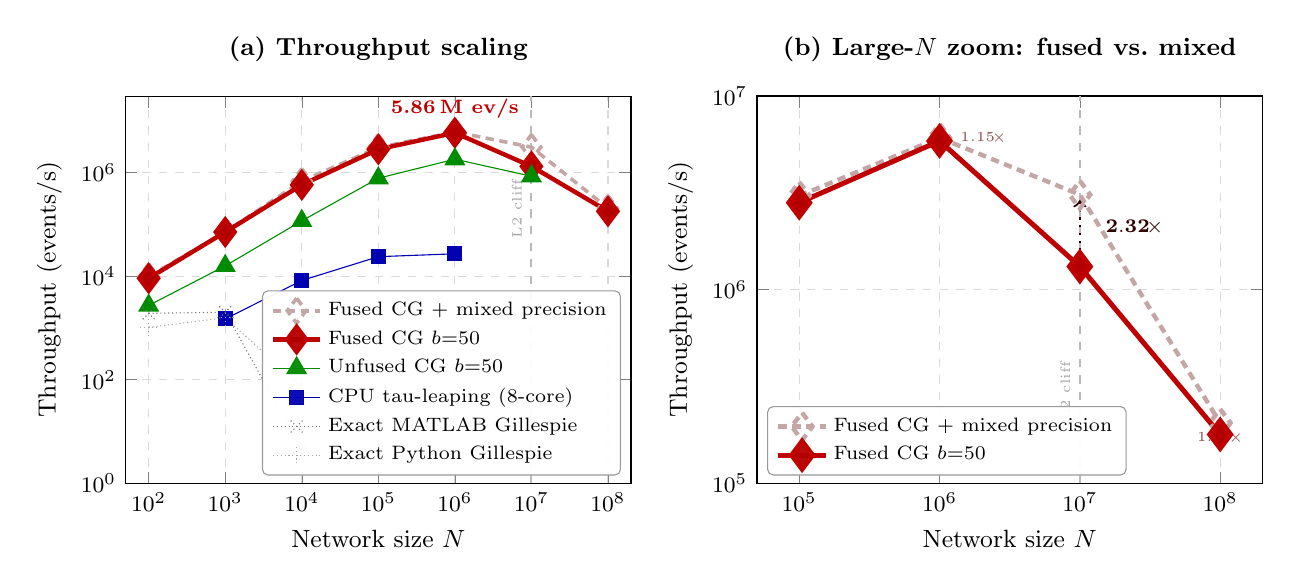
\begin{tikzpicture}

\begin{groupplot}[
    group style={
        group size=2 by 1,
        horizontal sep=1.6cm,
    },
    width=8cm, height=6.5cm,
    xmode=log, ymode=log,
    log basis x=10, log basis y=10,
    grid=major, grid style={dashed,gray!30},
    xlabel={Network size $N$},
    ylabel={Throughput (events/s)},
    xlabel style={font=\small},
    ylabel style={font=\small},
    xticklabel style={font=\footnotesize},
    yticklabel style={font=\footnotesize},
    title style={font=\small\bfseries, yshift=0.1cm},
    legend style={
        legend cell align=left,
        font=\scriptsize,
        fill=white, fill opacity=0.95, draw=black!40,
        text opacity=1, rounded corners=2pt,
    },
]

% ======================================================================
% LEFT PANEL: full scaling range (N = 10^2 .. 10^8). GPU "unfused
% eager" is dropped relative to the earlier draft — it is a purely
% pedagogical pre-CUDA-Graph baseline and its contribution is already
% captured by the CPU-to-CG gap; Section 5.5 discusses it in prose.
% ======================================================================
\nextgroupplot[
    xmin=50, xmax=2e8,
    ymin=1, ymax=3e7,
    xtick={1e2,1e3,1e4,1e5,1e6,1e7,1e8},
    xticklabels={$10^{2}$,$10^{3}$,$10^{4}$,$10^{5}$,$10^{6}$,$10^{7}$,$10^{8}$},
    ytick={1e0,1e2,1e4,1e6},
    yticklabels={$10^{0}$,$10^{2}$,$10^{4}$,$10^{6}$},
    title={(a) Throughput scaling},
    legend style={at={(0.98,0.02)}, anchor=south east},
]

% L2 cliff at N = 10^7
\draw[gray!55, dashed, line width=0.7pt]
    (axis cs:1e7, 1) -- (axis cs:1e7, 3e7);
\node[font=\tiny, color=gray!70, rotate=90, anchor=south]
    at (axis cs:1e7, 2e5) {L2 cliff};

% Fused CG + mixed precision (new; dashed pink)
\addplot[
    color=red!35!black!35!white, mark=diamond, mark size=4.5pt,
    line width=1.3pt, densely dashed,
] coordinates {
    (100,        9840.2)
    (1000,      71026.7)
    (10000,    683910.0)
    (100000,  3051268.9)
    (1000000, 6086231.9)
    (10000000, 3094503.4)
    (100000000, 205200.0)
};
\addlegendentry{Fused CG + mixed precision}

% Fused CG b=50 (headline, red diamonds)
\addplot[
    color=red!75!black, mark=diamond*, mark size=4.5pt,
    mark options={fill=red!70!black}, line width=1.6pt,
] coordinates {
    (100,       9091.8)
    (1000,     71096.0)
    (10000,   578859.8)
    (100000, 2813840.6)
    (1000000, 5860999.2)
    (10000000, 1316514.6)
    (100000000, 178800.0)
};
\addlegendentry{Fused CG $b{=}50$}

% GPU CUDAGraph (unfused) b=50 (green triangles)
\addplot[
    color=green!55!black, mark=triangle*, mark size=4pt,
    mark options={fill=green!55!black},
] coordinates {
    (100,       2717.4)
    (1000,     15795.8)
    (10000,   116776.2)
    (100000,  777103.9)
    (1000000, 1811158.3)
    (10000000, 849311.3)
};
\addlegendentry{Unfused CG $b{=}50$}

% CPU tau-leaping (8-core), derived from NUPS via the shared ratio
\addplot[
    color=blue!70!black, mark=square*, mark size=2.5pt,
    mark options={fill=blue!70!black},
] coordinates {
    (1000,     1491.0)
    (10000,    8253.0)
    (100000,  23767.0)
    (1000000, 27000.0)
};
\addlegendentry{CPU tau-leaping (8-core)}

% Exact MATLAB Gillespie
\addplot[
    color=black!55, mark=x, mark size=3pt, densely dotted,
] coordinates {
    (100,   1917.1)
    (1000,  2010.1)
    (10000,    4.5)
} node[pos=1, font=\tiny, below=1pt, black!55] {};
\addlegendentry{Exact MATLAB Gillespie}

% Exact Python Gillespie
\addplot[
    color=black!35, mark=+, mark size=3pt, densely dotted,
] coordinates {
    (100,   1026.7)
    (1000,  1577.0)
    (10000,   72.7)
};
\addlegendentry{Exact Python Gillespie}

% Headline annotation at N=10^6
\node[font=\scriptsize\bfseries, text=red!75!black, anchor=south]
    at (axis cs:1e6, 7.3e6) {5.86\,M ev/s};

% ======================================================================
% RIGHT PANEL: zoom on N \in [1e5, 1e8], only Fused CG and Fused CG +
% mixed precision. Visualises the L2-cliff divergence and the 2.32x
% post-cliff lift at N=10^7.
% ======================================================================
\nextgroupplot[
    xmin=5e4, xmax=2e8,
    ymin=1e5, ymax=1e7,
    xtick={1e5,1e6,1e7,1e8},
    xticklabels={$10^{5}$,$10^{6}$,$10^{7}$,$10^{8}$},
    ytick={1e5,1e6,1e7},
    yticklabels={$10^{5}$,$10^{6}$,$10^{7}$},
    title={(b) Large-$N$ zoom: fused vs.\ mixed},
    legend style={at={(0.02,0.02)}, anchor=south west},
]

\draw[gray!55, dashed, line width=0.7pt]
    (axis cs:1e7, 1e5) -- (axis cs:1e7, 1e7);
\node[font=\tiny, color=gray!70, rotate=90, anchor=south]
    at (axis cs:1e7, 3e5) {L2 cliff};

% Fused CG + mixed (top curve in zoom)
\addplot[
    color=red!35!black!35!white, mark=diamond, mark size=5pt,
    line width=1.6pt, densely dashed,
] coordinates {
    (100000,   3051268.9)
    (1000000,  6086231.9)
    (10000000, 3094503.4)
    (100000000, 205200.0)
};
\addlegendentry{Fused CG + mixed precision}

% Fused CG baseline
\addplot[
    color=red!75!black, mark=diamond*, mark size=5pt,
    mark options={fill=red!70!black}, line width=1.8pt,
] coordinates {
    (100000,  2813840.6)
    (1000000, 5860999.2)
    (10000000, 1316514.6)
    (100000000, 178800.0)
};
\addlegendentry{Fused CG $b{=}50$}

% Annotate speedup at N=10^6 and N=10^7 (the interesting points)
\node[font=\tiny\bfseries, text=red!35!black!70!white, anchor=west]
    at (axis cs:1.2e6, 6.1e6) {$1.15\!\times$};
\draw[->, thick, red!20!black, dotted]
    (axis cs:1e7, 1.45e6) -- (axis cs:1e7, 2.9e6);
\node[font=\scriptsize\bfseries, color=red!20!black, anchor=west]
    at (axis cs:1.3e7, 2.1e6) {$\mathbf{2.32\!\times}$};
\node[font=\tiny\bfseries, text=red!35!black!70!white, anchor=north]
    at (axis cs:1e8, 2.05e5) {$1.15\!\times$};

\end{groupplot}

\end{tikzpicture}
\end{document}
